
%%		but keep that option for other uses.

\documentclass[pdf-a,balance,colorlinks,upint,subscriptcorrection,varvw,mathalfa=cal=boondoxo, spanish,french,vietnamese,russian,greek]{asmeconf}
 \usepackage{amsmath}
 \usepackage{algorithm2e}
 \usepackage{algorithm}
 \usepackage{algpseudocode}
%%%%%  pdf metadata  %%%%%%%%%%%%%%%%%%%%%%%%%%%%%%%%%%%%%%%%%%%%%%%%%%%%%%%%%%%%%%%%%%%%%%%%%%%%%%%%%%

\hypersetup{%
	pdfauthor={John H. Lienhard},									  % <=== change to YOUR name
	pdftitle={ASME Conference Paper LaTeX Template},                  % <=== change to YOUR pdf file title
	pdfkeywords={ASME conference paper, LaTeX template, BibTeX style},% <=== change to YOUR pdf keywords
	pdfsubject = {Describes the asmeconf LaTeX template},			  % <=== change to YOUR subject
%	pdfurl={https://ctan.org/pkg/asmeconf},% may delete
	pdflicenseurl={https://ctan.org/pkg/asmeconf},% may delete
}


%========================================================================
% New Commands
%========================================================================
\newcommand{\todo}[1]{ {\color{red} TODO: #1} }
\newcommand{\blue}[1]{\textcolor{blue}{#1}}
\newcommand{\red}[1]{\textcolor{red}{#1}}
\newcommand{\hilight}[1]{\colorbox{yellow}{#1}}
\newcommand{\thetab}{\boldsymbol\theta}
\newcommand{\bs}{\boldsymbol}
%%%%%%%%%%%%%%%%%%%%%%%%%%%%%%%%%%%%%%%%%%%%%%%%%%%%%%%%%%%%%%%%%%%%%%%%%%%%%%%%%%%%%%%%%%%%%%%%%%%%%%%

\begin{document}

% Change these fields to the right content for your conference.
% You can comment these out if for some reason you don't want a header.
% Use title case (first letters capitalized), not all capitals

\ConfName{Proceedings of the ASME 2024\linebreak International Mechanical Engineering Congress and Exposition}
\ConfAcronym{IMECE2024}
\ConfDate{November 17--21, 2024} % update 
\ConfCity{Portland, OR} % update 
\PaperNo{IMECE2024-144618}

% Units of measure (e.g., cm) and other specialty lowercase terms in the title should be 
%   enclosed in \NoCaseChange{...} to maintain lower case type
%   LaTeX will automatically set the rest of the title in all capital letters.

\title{Chance Constrained PDE-Constrained Optimal Design Strategies Under High-Dimensional
Uncertainty} % <=== replace with YOUR title
%\title{Place Title Here: Place Subtitle After Colon} 
 
%   Put author names into the order you want. Use the same order for affiliations.
%   \affil{#} tags the author's affiliation to the address in \SetAffiliation{#}.
%   No space between last name and \affil{#}, separate names with commas.
%
%	For a sole author or a single affiliation for all authors, {#} may be left empty, as \affil{} and \SetAffiliation{} (but not with [grid] option!)
%
%   \CorrespondingAuthor{email} follows that author's affiliation, no spaces.  
%   If multiple corresponding authors, put both email addresses in the same command and place after both authors.
%
%   \JointFirstAuthor, if applicable, follows the affiliation of the relevant authors, no spaces.

\SetAuthors{%
	Pratyush Kumar Singh \affil{1},  
	Danial Faghihi\affil{1}\CorrespondingAuthor{danialfa@buffalo.edu}
	}

\SetAffiliation{1}{University at Buffalo, Buffalo, NY }
%	Note: Luis and Maria are not real people.  Henry and Catherine have been dead for >450 years.

%	To switch from inline author names to gridded names, use the [grid] option.

\maketitle

%%% Use this footnote for tracking various versions of your draft. Change text to suit your own needs. 
%%% \date{..} calls the same command. 
%\versionfootnote{Documentation for \texttt{asmeconf.cls}: Version~\versionno, \today.}% <=== Delete before final submission.

%%% Change these to your keywords.  Keywords are automatically printed at the end of the abstract.
%%% This command MUST COME BEFORE the end of the abstract.
%%% If you don't want keywords, leave the argument of \keywords{} empty (or use the abstract* environment)

\keywords{Optimization under uncertainty, Chance constraint, Thermal breaks}

%%%%%  End of fields to be completed. Now write your paper. %%%%%%%%%%%%%%%%%%%%%%%%%%%%%%%%%%%%%%%%%%%


%%%%%  ABSTRACT  %%%%%%%%%%%%%%%%%%%%%%%%%%%%%%%%%%%%%%%%%%%%%%%%%%%
%%
%% Abstract should be 200 words or less
\begin{abstract}
\noindent
This study focuses on developing a computational framework for model-based design of the
thermal insulation elements of net-zero buildings based on silica aerogel porous materials,
ensuring they provide superinsulation while upholding structural integrity. This approach
employs a multiphase continuum model, capturing the thermomechanical properties of the
insulation component through a set of partial differential equations (PDE). The framework
considers the uncertainty associated with both the physical parameters like elasticity and
thermal conductivity for the solid and fluid phases, as well as the design parameter, which is
the spatial distribution of the aerogel porosity over the domain of the component. The
combination of spatially varying design and uncertainty parameters, along with their finite
element discretization, results in a high dimensional PDE-constrained optimal design problem.
A mean cost functional is implemented to achieve both target insulation performance and
uncertainty reduction during the design process. To avoid stress concentration in the
component, chance constraints are included in the optimization formulation, which ensures that the probability of a function that measures the difference between evaluated stress from the multiphase model and a critical threshold value lies within tolerance.
A scalable method is introduced for solving PDE-constrained optimization under
uncertainty that is both efficient and dimension-independent. For efficiency, this method
exploits a second-order Taylor approximation of the design objective and chance constraint function, which solves a generalized eigenvalue problem. Combined with a gradient-based optimization built on Lagrangian formulation, it results in dimension-independent (scalable) computational costs.
The numerical experiments on the design of thermal breaks of the buildings demonstrate that the proposed framework leads to a significant reduction in computational cost while preserving thermal insulation performance and avoiding mechanical failure due to stress concentration.

\end{abstract}

%----------------------------------------------------------------------------------------------------------------------------
%--------------------------------------------------------Introduction--------------------------------------------------------

\section{Introduction}
\noindent
Thermal breaks play a pivotal role in net-zero buildings by intercepting the path of heat transfer and mitigating the adverse effects of thermal bridging, thereby significantly reducing energy consumption. Silica aerogels, characterized by their lightweight nature and ultra-low thermal conductivity, are poised to revolutionize the next generation of thermal break materials.
However, their intrinsic limitation lies in their low mechanical strength, posing a barrier to their widespread adoption in practical applications. Recent advancements in additive manufacturing, particularly the direct ink writing method, offer a promising avenue for addressing this challenge. This method enables the fabrication of components with diverse geometries and spatially varying properties to enhance the aerogel's mechanical properties and expand its functional capabilities.
In the context of thermal breaks, high-porosity aerogels exhibit exceptional thermal insulation performance, while low-porosity variants are essential for imparting the necessary mechanical robustness to withstand external loads. Achieving this thermo-mechanical balance necessitates the adoption of simulation-based design methods \cite{chen2013weighted,chen2019taylor,chen2021taylor,tan2024scalable}, aimed at developing cost-effective components with superior insulation properties and requisite mechanical stability.


This paper presents an efficient computational framework for the optimal design of thermal break components subject to partial differential equation (PDE) constraints and high-dimensional uncertainty, focusing specifically on the spatial distribution of the silica aerogel porosity.
The forward PDE model employed herein relies on a two-phase thermo-mechanical model of aerogel based on the continuum theory of mixtures. The design parameter under consideration is the spatial distribution of porosity across the domain, which inherently exhibits spatially correlated uncertainty stemming from material variations and fabrication errors.
The optimization objective involves minimizing the mean of the uncertain thermal insulation performance. To ensure the mechanical integrity of the component, chance constraints are imposed on the optimization problem \cite{chen2019taylor,chen2021taylor}, limiting the maximum von Mises stress induced in the domain to a specified threshold below the critical stress level, thus averting mechanical failure due to excessive stress.
To develop a computationally efficient solution algorithm, a second-order Taylor approximation is employed to linearize the optimization cost function and chance constraint. These linearizations leverage the action of the Hessian on a set of random directions, employing a randomized algorithm to solve the associated generalized eigenvalue problem.
The optimization procedure is grounded in a gradient-based approach formulated within the Lagrangian framework, ensuring scalability by requiring only a modest number of vectors and their gradients for constructing the design gradient. This results in a framework with computational cost scalability that is independent of the dimensionality of the design parameters.
Numerical experiments conducted on thermal breaks for buildings demonstrate that the proposed framework yields a substantial reduction in computational cost compared to Monte Carlo-based estimations of objective function moments and chance constraints.

The structure of the paper is as follows: Section 2 depicts the optimization problem under uncertainty, encompassing the forward model, specification of design and uncertain parameters, and representation of the design objective. Section 3 is devoted to detailing the scalable framework for PDE-constrained chance-constrained optimal design, outlining the Taylor approximation of both the mean cost functional and chance constraint function. In Section 4, the gradient-based optimization method is expounded upon, including the assessment of the cost functional and its gradient concerning design parameters. Section 5 presents the numerical findings regarding optimal design, succeeded by the concluding remarks in Section 6.


%-----------------------------------------------------------------------------------------------------------------------------
%--------------------------------------------------------Forward Model--------------------------------------------------------
\section{Forward Model}
\noindent
The forward model is based on the continuum mixture theory \cite{tan2022predictive}. The model considers two phases which are the incompressible solid aerogel and compressible fluid phases between the materials.  The governing equations at steady state for the thermal and mechanical parts can be described using the following PDEs,
%-------------Defining PDEs--------------%
\begin{equation}\label{multiphase}
%\begin{split}
    - \nabla \cdot ( \phi_s \kappa_s \nabla \theta_s) = - h(\theta_s - \theta_f) \: 
%\end{split}
\end{equation}
\begin{equation}
    - \nabla \cdot ( \phi_f \kappa_f \nabla \theta_f) = h(\theta_s - \theta_f) \: 
\end{equation}
\begin{equation}
    D p = -( \nabla \cdot \boldsymbol{u_{s}}) \:
\end{equation}
\begin{equation}\label{multiphase_end}
    \nabla . \boldsymbol{T_{s}}^{'} + (2 \phi_f - 1) \nabla p = 0 \:
\end{equation}
where model parameters are $\boldsymbol{\theta}= (\kappa_s, \kappa_f, D, \boldsymbol{E_{s}})$ and states are $\boldsymbol{u} = ( \theta_s, \theta_f, \boldsymbol{u_{s}}, p)$. The state variables $\theta_s, \theta_f, \boldsymbol{u_{s}}$ and $p$ represent the solid and fluid temperatures, solid displacement, and fluid pressure respectively over the whole domain. The stress tensor is defined as $\boldsymbol{T'} = 2 \mu \boldsymbol{E_{s}} + \lambda \: tr(\boldsymbol{E_{s}})\boldsymbol{I}$ with $\boldsymbol{E_{s}} = \frac{1}{2} (\nabla \boldsymbol{u_{s}} + (\boldsymbol{u_{s}})^{T})$ where $\boldsymbol{E_{s}}$ is the solid strain and $\lambda$ and $\mu$ are the Lame constants.


Due to the imprecise control of the aerogel ink properties, there is an uncertainty associated with the porosity value within the aerogel thermal break.
The uncertain parameter $m$ is represented by a Gaussian measure $\mu = \mathcal{N}(\overline{m},\mathcal{C})$ with mean $\overline{m}$ and covariance $\mathcal{C}$, which can be represented by a Matern covariance kernel such that $\mathcal{C} = \mathcal{A}^{-2}$ \cite{lindgren2011explicit}. 
The design parameter $d(\boldsymbol{x}) \in [0, 1]$ is related to the uncertain and spatially-correlated fluid volume fraction (porosity) $\phi_f(\boldsymbol{x})$, through $\phi_f(\boldsymbol{x}) = g(d(\boldsymbol{x}) + m(\boldsymbol{x}))$, where $g(\cdot)$ is a linear map.
Finally, the design objective is defined as thermal compliance of the insulation system as, 
\begin{equation}
    Q = \frac{1}{2} \sum_{i=s,f} {\langle \phi_i \kappa_i \nabla \theta_i,  \nabla \theta_i \rangle}_{\Omega}  + \sum_{i=s,f}  {\langle \phi_i h_{air} (\theta_i - \theta_{amb}), \theta_i \rangle }.
\end{equation}
%--------------------------------------------------------------------


%----------------------------------------------------------------------------------------------------------------------------------
%--------------------------------------------------------Scalable Framework--------------------------------------------------------
\section{Scalable Framework for Chance Constraint Optimal Design}
\noindent
The PDE-constrained optimization under uncertainty problem aims to determine the spatial distribution of porosity within the thermal break, which avoids stress concentration and provides thermal performance. 
%
The PDE  (\ref{multiphase}) can be abstractly represented as $\mathcal{R}(u,m,d) = 0 \: \text{in} \: \mathcal{V}^{'}$,
where $m \in \mathcal{M}$ denotes an uncertain parameter field residing in a Banach space $\mathcal{M}$ and has a probability distribution $\mu$.
To incorporate the uncertainty stemming from the dependence on $m$ into the design process, we use the mean of design objective in the cost functional as,
    \begin{equation}\label{mean cost functional}
        \mathcal{J}(d) = \mathbb{E}[Q(m,d)] + R(d), 
    \end{equation}
where the term $R(d)$ represents the regularization term. In this work, we considered Tikhonov regularization, which can be expressed as,
\begin{equation*}
    R (d) = \int_{\Omega}  \beta_{tik} {|\nabla d|}^2  \,d \Omega, 
\end{equation*}
where $\beta_{tik}$ is the parameter that controls the interface thickness.
To mitigate the risk of stress concentration within the domain, it is imperative that the maximum stress remains below the critical stress threshold. However, due to the non-differentiable nature of the maximum stress, direct optimization poses significant challenges. This can be resolved using stress aggregation function based on p-norm \cite{le2010stress}, which is a smooth approximation of the maximum stress facilitating the application of gradient-based optimization techniques.
For the chance constraint function, we consider the p-norm of the von Mises stress for the component, which approximates its maximum value in the entire domain. The p-norm for the von mises stress can be computed as
\begin{equation}
    T_{\text{pn}} = {\left( \int_{\Omega} T_{\text{VM}}^{p} \,d \Omega \right)}^{\frac{1}{p}}
\end{equation}
The chance constraint function can hence be written as,
\begin{equation}
    f = T_{cr} - T_{\text{pn}},
\end{equation}
where $T_{cr}$ is the limiting critical stress and 
$T_{\text{pn}}$ is the p-norm of the von Mises stress over the domain.
To avoid stress concentration, we consider a chance constraint:
%
    \begin{equation} \label{inequality chance}
        P(f(m,d) \geq 0) \leq \alpha_{c},
    \end{equation}
%
    for a critical chance $0 < \alpha_{c} <1$.
    The probability is given by 
    \begin{eqnarray}
        P(f(m,d) \geq 0) & = & \mathbb{E}[\mathbb{I}_{[0,\infty]} (f(m,d))] \nonumber\\
        & = & \int_{\mathcal{M}} \mathbb{I}_{[0,\infty]} (f(m,d)) \, d \mu(m),
    \end{eqnarray}
    where $\mathbb{I}_{[0,\infty]} (f(m,d))$ is an indicator function defined as:
    \[
 \mathbb{I}_{[0,\infty]} (f(m,d)) =
\begin{cases}
  1 & \text{if } f(m,d) \geq 0 \\
  0 & \text{if } f(m,d) < 0 \\
\end{cases}
\]
Hence, the PDE-constrained optimization can be written as,
 \begin{equation}
     \underset{d}{\text{min}} \: \mathcal{J}(d) \: \text{subject to \eqref{multiphase}-\eqref{multiphase_end} and chance constraint \eqref{inequality chance}}.
 \end{equation}
 
%--------------------------------------------------------------------------------------------------------------------
%-----------------------------------Taylor approximation-------------------------------------------------------------
\subsection{Taylor Approximation}
\noindent
Due to the requirement of large PDE evaluations in the sample averaged calculation of the mean in the cost functional, Taylor approximation is applied for both the objective function and the constraint function, which requires an efficient eigenvalue decomposition of the Hessian of the objective and constraint functions with respect to the random parameter field.
We assume that the objective function $Q$ can be approximated as a second-order Taylor expansion centered around the mean of the uncertain parameter $\overline{m}$, which is given by
\begin{equation}
    T_{2} Q(m,d) = \sum_{k=0}^2 \partial_{m}^k Q(\overline{m},d) (m - \overline{m})^{k}
\end{equation}
The closed form for the expectation of the quadratic Taylor approximation $\mathcal{J}_{quad}$ is defined as:
\begin{equation}\label{eq:taylor objective}
    \mathcal{J}_{quad} = \mathbb{E}[T_2 Q(d)] = Q(\overline{m},d) + \frac{1}{2} tr(\overline{\mathcal{H}}_q)
\end{equation}
where $tr(\overline{\mathcal{H}}_q)$ represents the trace of $\mathcal{H}_{q}$ which is the covariance-preconditioned Hessian of the objective Hessian $Q$. The eigenvalues $\lambda_n$ are obtained by solving the following generalized eigenvalue problem,
\begin{equation} \label{eigen}
    \langle \zeta, \nabla^{2}_{mm}Q \: \psi_j \rangle = \lambda_j \langle \zeta, \mathcal{C}^{-1} \psi_j \rangle, \: \forall \zeta \in \mathcal{M},\: j = 1,....,N_{eig} 
\end{equation}
where the eigenvectors $\psi_j$ exhibit orthonormality with $\mathcal{C}^{-1}, \langle \psi_i, \mathcal{C}^{-1} \psi_j \rangle = \delta_{ij},i,j = 1,...N_{eig}$ and $\delta_{ij}$ denote the Kronecker delta function. 
Using an n-degree finite element discretization, \ref{eigen} can be written as $\boldsymbol{A \psi =} \lambda \boldsymbol{B \psi}$. 
%
The eigenvalue problem at hand can be effectively solved using a double-pass randomized algorithm \cite{Saibaba}. Subsequently, the obtained eigen-decomposition is employed to estimate the trace of the covariance-preconditioned Hessian $\mathcal{H}_q$ via its dominant eigenvalues $\lambda$, expressed as,
\begin{equation}
        tr(\overline{\mathcal{H}_q}) = \sum_{n=1}^{N_q} \lambda_{n},
\end{equation}
where, $N_{q}$ represents the low-dimensional dominant modes. As demonstrated in the results section, $N_{q}$ is invariant to the parameter dimension, and the eigenvalues exhibit rapid decay for numerous problems when the covariance-preconditioned Hessian is low-rank.


We construct a second-order Taylor expansion of the constraint function $f$ at $\overline{m}$ similar to \eqref{eq:taylor objective} denoted by $T_{2}f$ to facilitate approximation of the probability $P(f(m,z)\geq 0)$ through sampled averaged approximation as:
\begin{equation}\label{eq: taylor constraint}
    P(f(m,d))\geq 0) \approx f_{M}^{2}(d) = \frac{1}{M_{f}} \mathbb{I}_{[0,\infty)}(T_{2}f(m_{i},d)).
\end{equation}
%
This approximation of the constraint function obviates the necessity for a large number of PDE solves to assess the probability utilizing sample averaging methods.




%-------------------------------------------------------------------------------
%----------------------------Gradient based optimization------------------------
\section{Gradient-based optimization}
\noindent
A gradient-based approach is employed to tackle the chance-constrained optimization problem outlined in the preceding section. Specifically, the Newton Conjugate Gradient algorithm is employed, which constitutes a modified variant of Newton's method. This algorithm leverages the conjugate gradient technique to compute the inverse of the local Hessian matrix.
The optimization process necessitates the incorporation of four key components: (1) a smooth approximation of the indicator function, (2) a penalty method for handling inequality chance constraints, (3) a continuation scheme to refine both the smooth approximation and the penalty term associated with inequality chance constraints, and (4) the calculation of the gradient of the quadratic approximate cost functional $\mathcal{J}_{quad}$.
This section elaborates the entire methodology to solve the optimization problem.

\subsection{Smooth approximation}
\noindent 
The indicator function utilized in the chance constraint exhibits discontinuity at $f(m,d) = 0$. In order to employ a gradient-based optimization method, this discontinuous indicator function must be approximated with a smooth, continuous counterpart. One approach involves employing a logistic function as a smooth approximation of the indicator function such that,
\begin{equation}
    \mathbb{I}_{[0,\infty]}(x) \approx l_{\beta}(x) = \frac{1}{1 + e^{-2 \beta x}},
\end{equation}
where a larger $\beta$ corresponds to a sharper transition at $x=0$.

\subsection{Penalty Method}
\noindent 
To impose the inequality constraint \eqref{inequality chance}, a quadratic penalty method \cite{nocedal2006quadratic} is applied. The quadratic penalty function is defined as,
\begin{equation}
        S_{\gamma}(x) = \frac{\gamma}{2}{(max{\{0,x\}})}^2
\end{equation}
where $\gamma > 0$ is a constant corresponding to the weight of the penalty. Using the penalty method, the chance-constrained problem can be rewritten as
\begin{equation}\label{eq: optimization_penalty}
    \underset{d \in [0,1]}{min} \mathcal{J}(d) + \mathcal{S}_{\gamma}(\mathbb{E}[l_\beta(f)] - \alpha_c)  
\end{equation}
Let $\mathcal{J}(d)$ denote the approximation of the cost functional in \eqref{mean cost functional}, and $\nabla_{d} \mathcal{J}$ denote the gradient of cost functional with respect to design variable. A continuation scheme \cite{chen2021taylor} is utilized, which gradually increases the smoothing parameter $\beta$ and penalty parameter $\gamma$ inside an outer loop and Newton Conjugate Gradient optimizer. 
%---------------------------------Adaptive Optimization-----------------------------------------------
%-----------------------------------------------------------------------------------------------------
\subsection{Adaptive optimization}
\noindent
The gradient-based scheme uses a continuation scheme that gradually increases the smoothing parameter $\beta$ and penalty parameter $\gamma$ to achieve convergence \cite{chen2021taylor}. An initial value of the smoothing parameter $\beta_{0}$ and the penalty parameter $\gamma_{0}$ is defined for the continuation scheme. These parameters are updated at the end of each iteration using scaling parameters $\sigma_{\beta}$ and $\sigma_{\gamma}$ for smoothing and penalty parameters, respectively. For $k^{th}$ iteration , the updated smoothing parameter is $\beta_{k+1} = \sigma_{\beta} \beta_{k}$ and the updated penalty parameter is $\gamma_{k+1} = \sigma_{\gamma} \gamma_{k}$. In an outer loop, we update the parameters $\beta$ and $\gamma$, whereas a Newton Conjugate Gradient (Newton CG) is applied in the inner loop to solve the optimization problem \eqref{eq: optimization_penalty}. The stopping criterion for the outer loop is if the maximum number of iterations $k_{\text{max}}$ is reached. For each iteration, the approximated chance is computed through the quadratic approximation $f_{M}^{2}$ of the chance function as given in (\ref{eq: taylor constraint}). The output is the optimal value of design parameter $d_{\text{opt}}$. The algorithm for this adaptive optimization is given in Algorithm 1.
\begin{algorithm}[H]
    \textbf{Algorithm 1}\\
    \textbf{Input:} $d_{0}, \beta_{0}, \gamma_{0}, \sigma_{\beta}, \sigma_{\gamma}, \hat{f}= f_{M}^{2}(d)$\\
    \textbf{while} $||d_{k} - d_{k-1}|| \leq \mathcal{\epsilon_{\text{out}}}$ or $k<k_{\text{max}}$\\
    1. $d_{k+1} = \text{Newton CG}(d_{k},\mathcal{J}(d), \nabla_{d} \mathcal{J} (d), \epsilon_{\text{in}})$.\\
    2. Evaluate approximate chance $\hat{f}_{k+1}$ at $d_{k+1}$.\\
    3. Update $\beta_{k+1} = \sigma_{\beta} \beta_{k}$, $\gamma_{k+1} = \sigma_{\gamma} \gamma_{k}$\\
    \textbf{end while}\\
    return $d_{\text{opt}}$
\end{algorithm}

\subsection{Computation of gradient of cost functional}
\noindent
The gradient and Hessian of design objective $Q$ with respect to uncertain parameter $m$ are known as $m_{Q}$-gradient and $m_{Q}$-Hessian; also, the gradient and Hessian of constraint function $f$ with respect to  $m$ are known as $m_{f}$-gradient and $m_{f}$-Hessian. 
An approximate cost functional using Taylor approximation and its gradient with respect to the design variable is computed using a gradient-based algorithm. Lagrangian formulation is employed to derive the gradient of the quadratic approximation of the design objective $\mathcal{J}_{quad}$ with respect to the design parameter $d$ denoted as $d$-gradient. A Lagrangian functional is created by enforcing all the PDE constraints.  Setting the variation of Lagrangian as zero with respect to state variables, adjoint variables, and eigenvalues, we can come up with a set of incremental state problems, incremental adjoint problems, linear state problems, and linear adjoint problems. The algorithm for computing the $d$-gradient is given in Algorithm 2.
\begin{algorithm}[H]
    \textbf{Algorithm 2}\\
    1. Solve for $m_{Q}$-gradient and $m_{Q}$-Hessian\vspace{0.03 in}\\
    2. Solve for $m_{f}$-gradient and $m_{f}$-Hessian.\vspace{0.03 in}\\
    3. Solve for generalized eigenpairs with double-pass randomized algorithm.\vspace{0.03 in}\\
    4. Compute approximate cost functional $\mathcal{J}_{quad}$ by \eqref{eq:taylor objective}\\
    5. Solve the linear state problem.\vspace{0.03 in}\\
    6. Solve the linear adjoint problem.\vspace{0.05 in}\\
    7. Obtain the $d$-gradient. 
\end{algorithm}


%-------------------------------------------------------------------------------------------------------
%-------------------------------------Numerical Results-------------------------------------------------
\section{Results and Discussions}
\noindent
This section presents numerical experiments conducted on an insulation component with the objective of maximizing thermal insulation performance while ensuring adequate mechanical stability through the incorporation of chance constraints. The numerical results aim to assess the impact of critical chance, limiting critical stress value, Tikhonov regularization weight, smoothing, and penalty parameters.
The problem under consideration entails an L-shaped geometry. For the heat transfer model, Neumann boundary conditions are imposed, with ambient temperatures set at 1 and 0 at the outer and inner boundaries, respectively, and insulated conditions applied to the remaining two boundaries. The boundary conditions of the mechanical model involve prescribing a uniform traction load with magnitude 1 along and in the opposite direction of the unit vectors on the outer boundary, fixing solid displacement on the inner boundary, and applying roller conditions to the other boundaries.
Model parameters are specified as $\kappa_s=0.477$, $\kappa_s=0.085$, $h=81059$, $C=0.25$, $\lambda=6.77$, and $\mu=3.38$, adopted from the previous research \cite{tan2022predictive}. The uncertain parameter $m$ is the Gaussian random field with Matern covariance and mean $\overline{m}=0$ and correlation length $L_{C} = 0.02$. Figure \ref{fig:m_sample} shows some samples of the uncertain parameter used in the numerical experiments.
\begin{figure}[h]
\centering
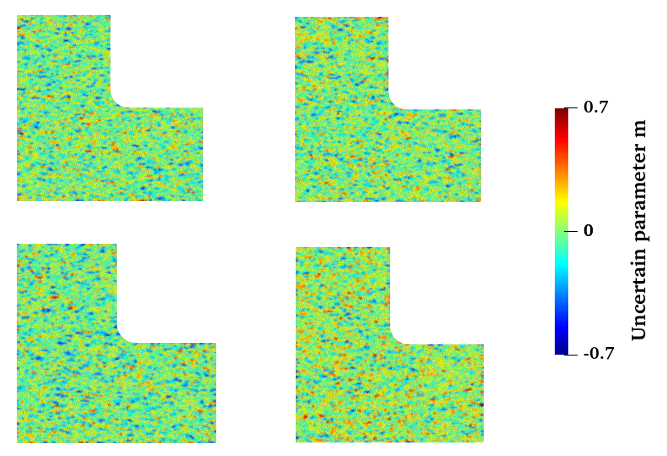
\includegraphics[width=1\linewidth]{Figures/m_sample.png} 
\caption{Samples of uncertain parameter $m$ with correlation length $L_{C} = 0.02$\label{fig:m_sample}}
\end{figure}
\begin{figure}[h]
\centering
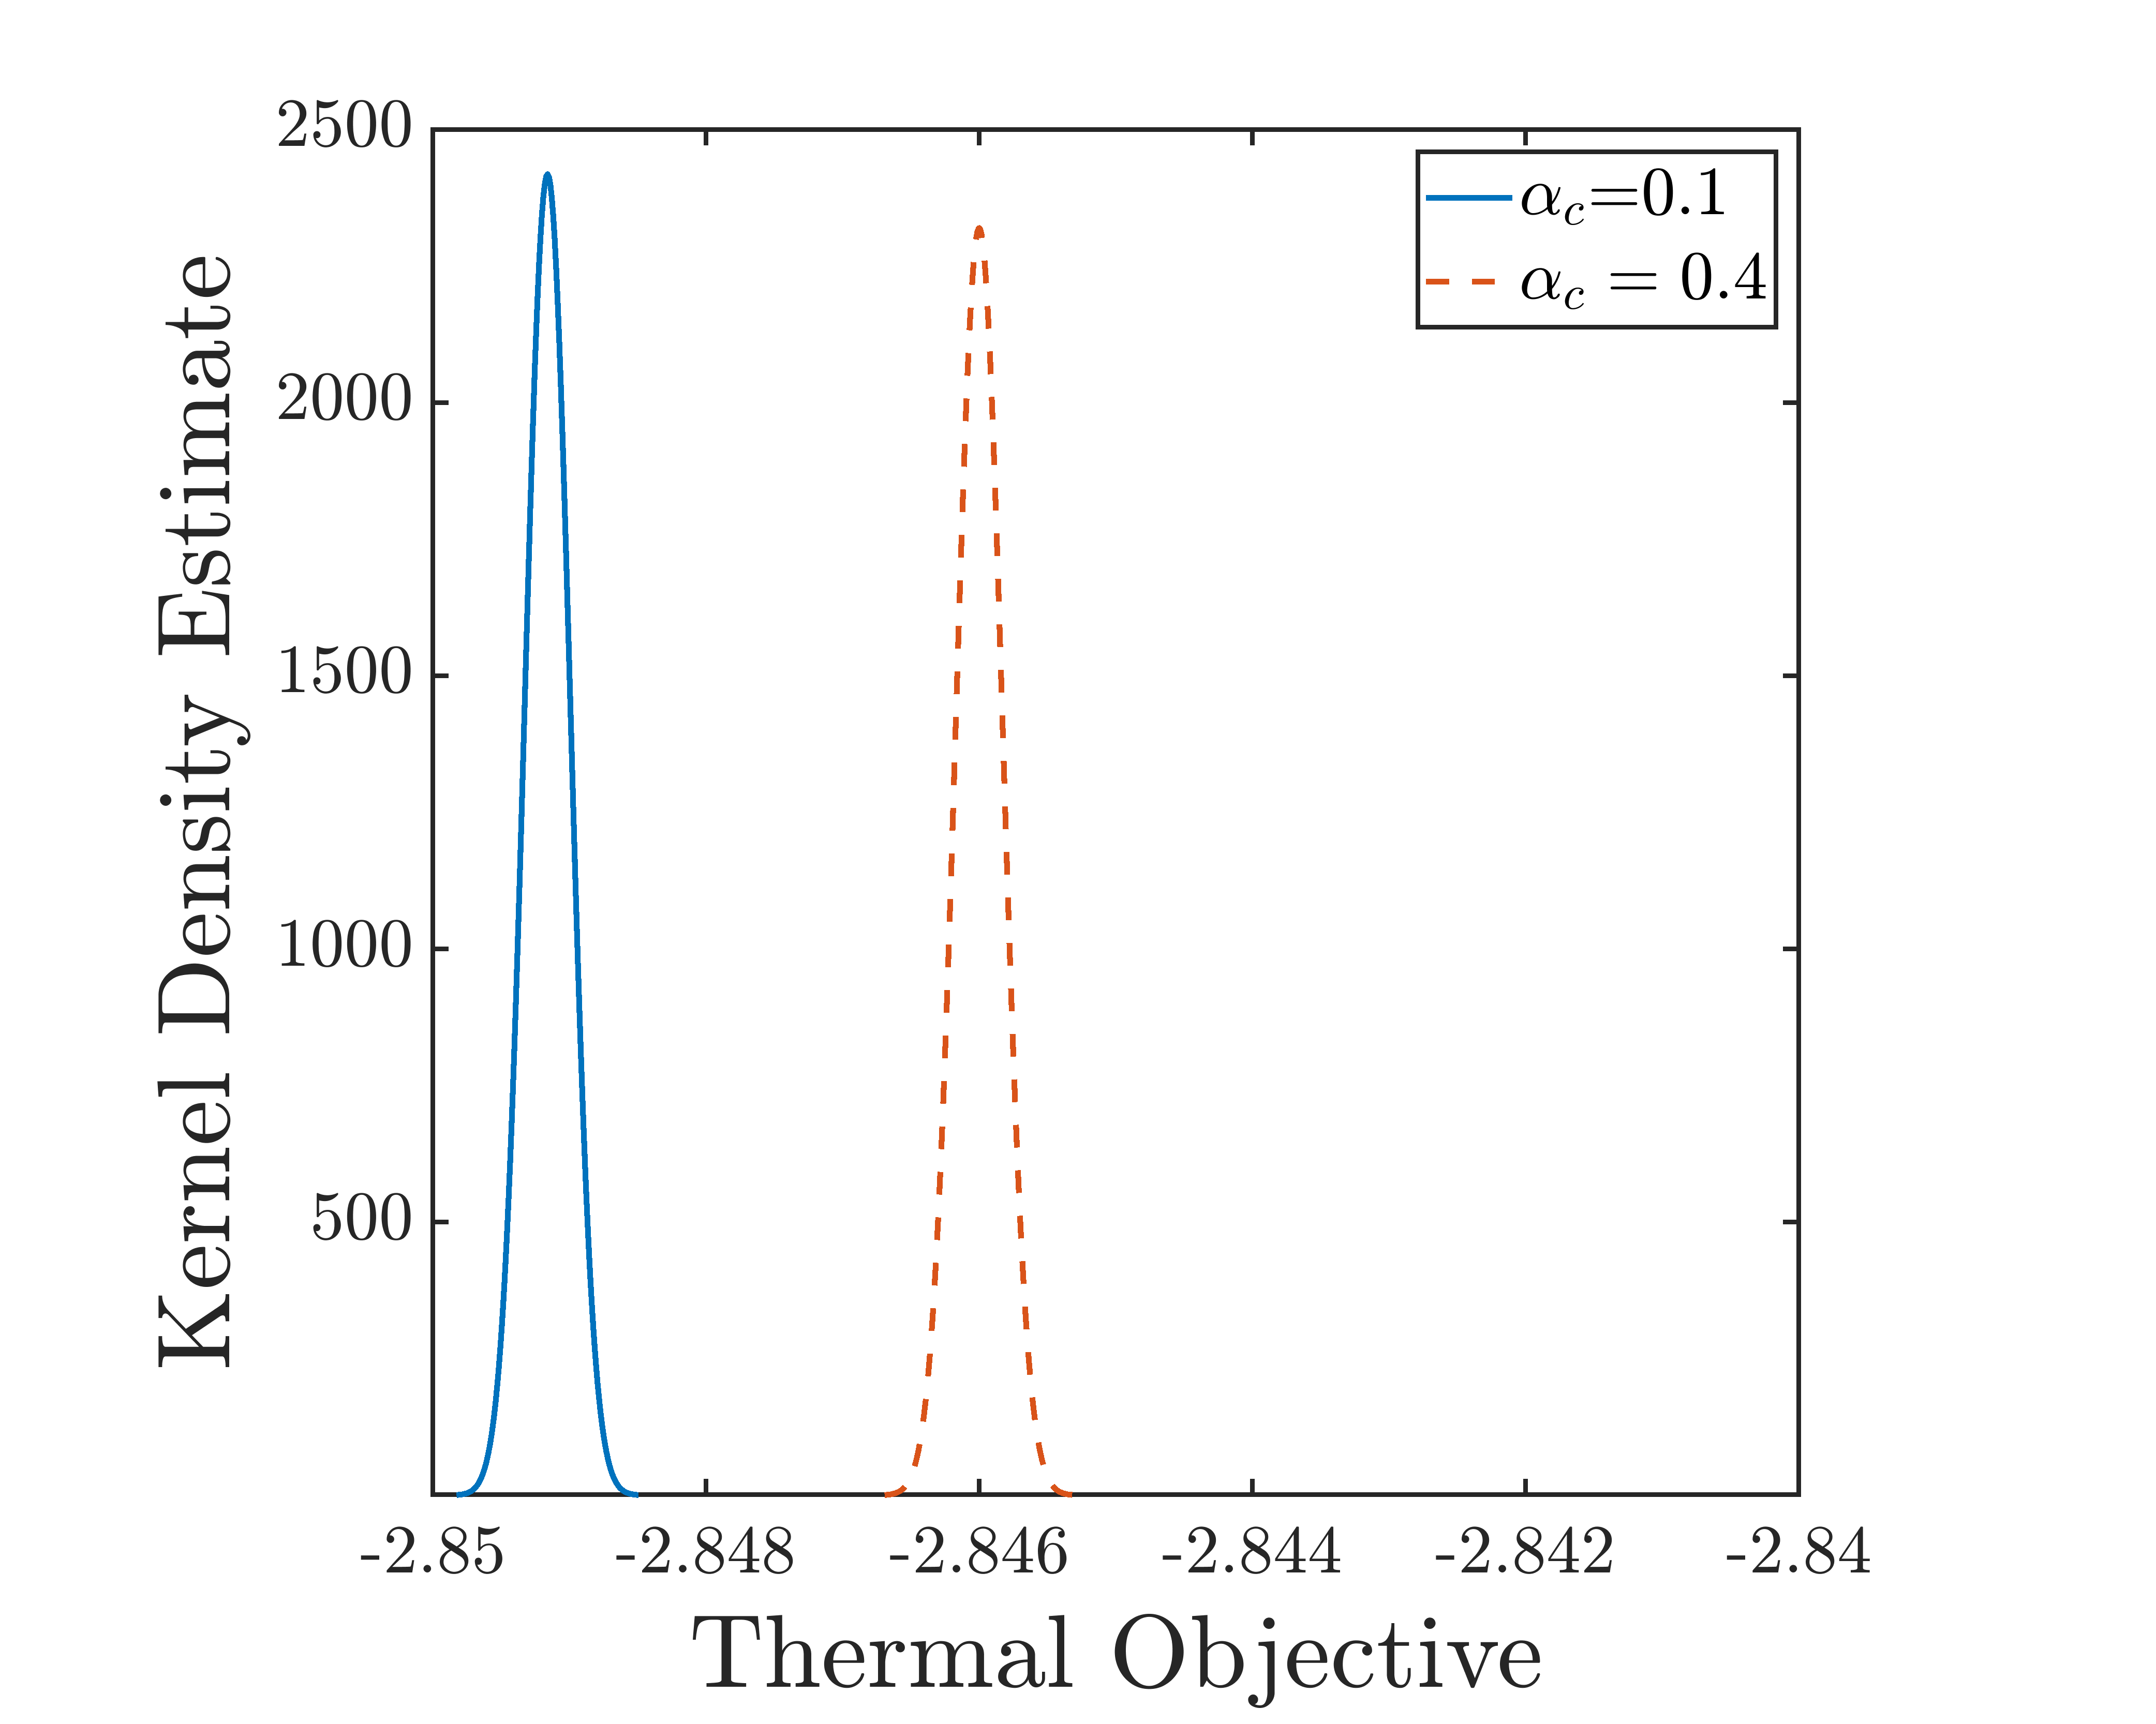
\includegraphics[width=0.8\linewidth]{Figures/Thermal_objective.png} 
\caption{The probability distribution of the thermal objective Q for the designed components at different values of $\alpha_{c}$}\label{fig:chance_thermal}
\end{figure}
\begin{figure}
\centering
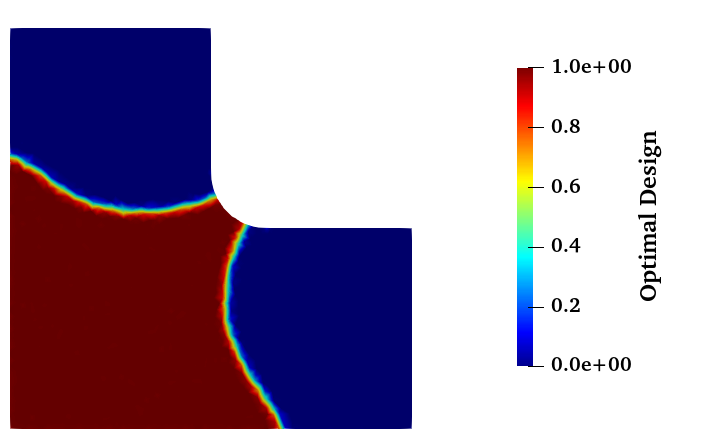
\includegraphics[width=0.44\linewidth]{Figures/Pattern_1.png} ~ 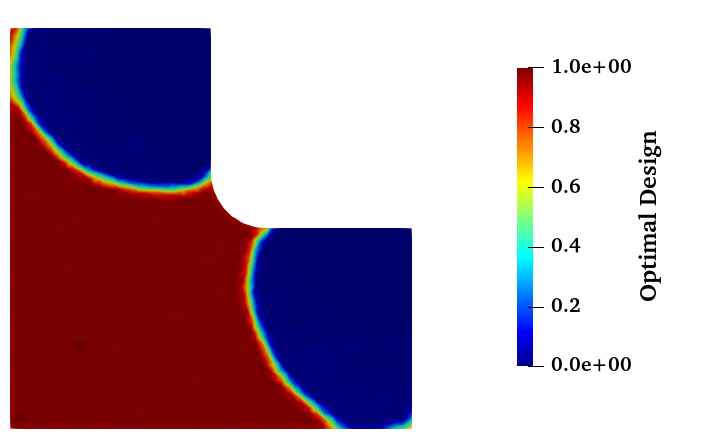
\includegraphics[width=0.44\linewidth]{Figures/Pattern_2.png} \vspace{0.2 in}\\
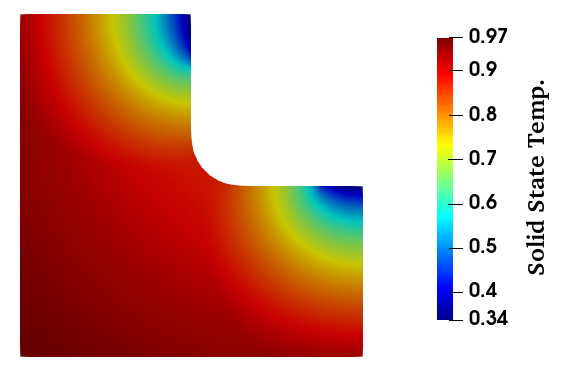
\includegraphics[width=0.44\linewidth]{Figures/Solid_temp_1.png} ~ 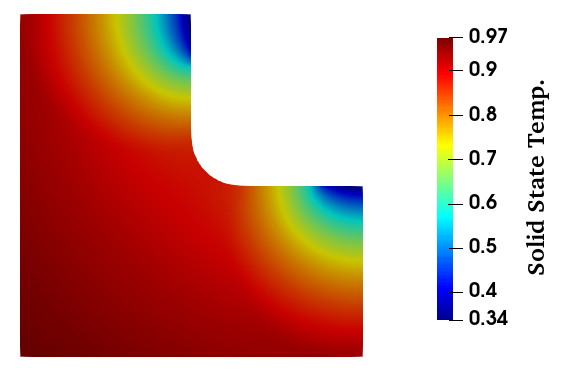
\includegraphics[width=0.44\linewidth]{Figures/Solid_temp_2.png}\vspace{0.2 in}\\
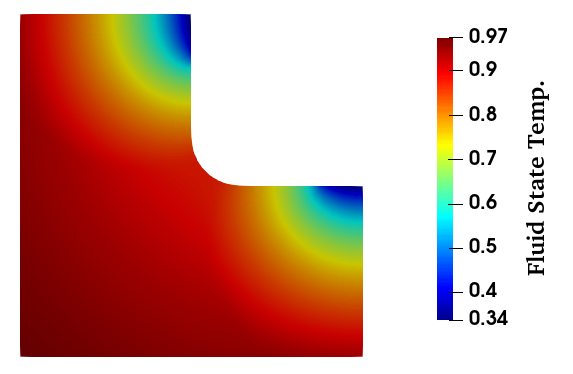
\includegraphics[width=0.44\linewidth]{Figures/Fluid_Temp_1.png} ~ 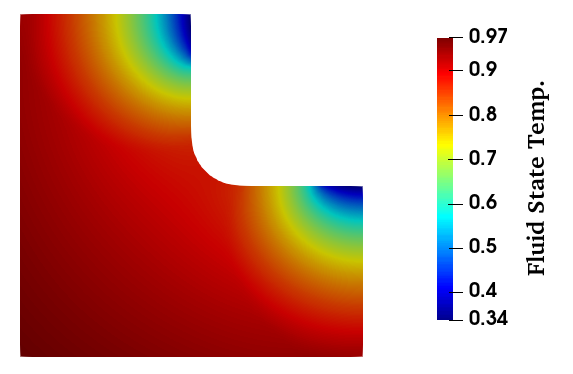
\includegraphics[width=0.44\linewidth]{Figures/Fluid_temp_2.png}\vspace{0.2 in}\\
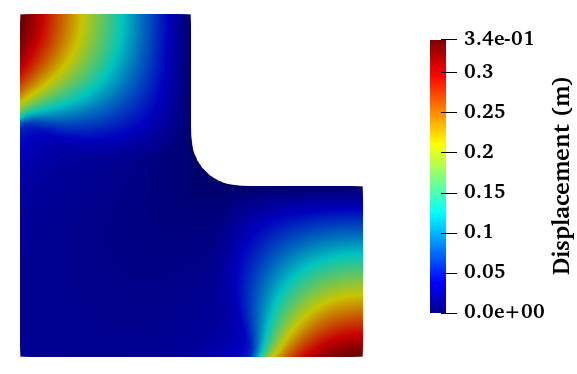
\includegraphics[width=0.44\linewidth]{Figures/Displacement_1.png} ~ 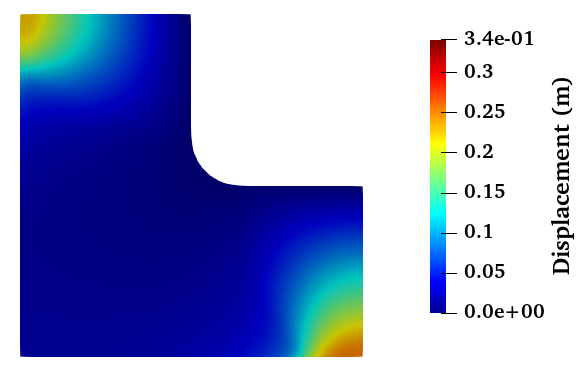
\includegraphics[width=0.44\linewidth]{Figures/Displacement_2.png}\vspace{0.2 in}\\
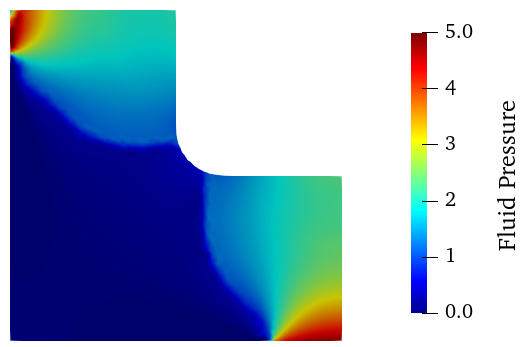
\includegraphics[width=0.44\linewidth]{Figures/Pressure_1.png} ~ 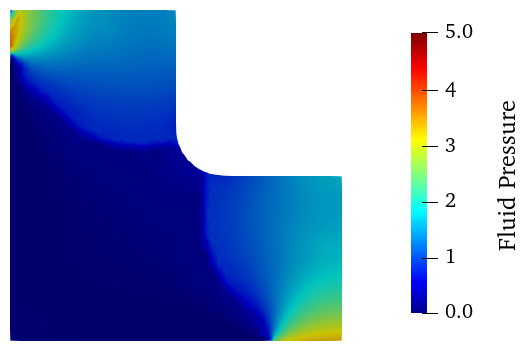
\includegraphics[width=0.44\linewidth]{Figures/Pressure_2.png}\vspace{0.2 in}\\
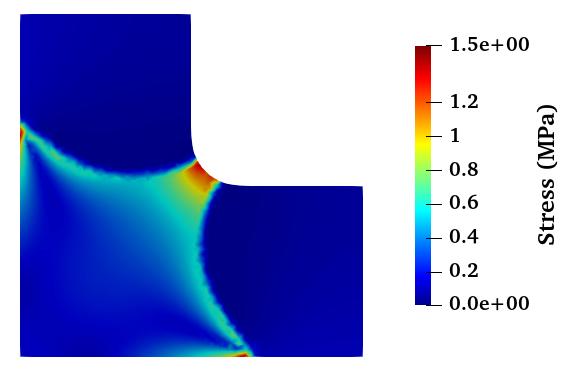
\includegraphics[width=0.44\linewidth]{Figures/Stress_VM_1.png} ~ 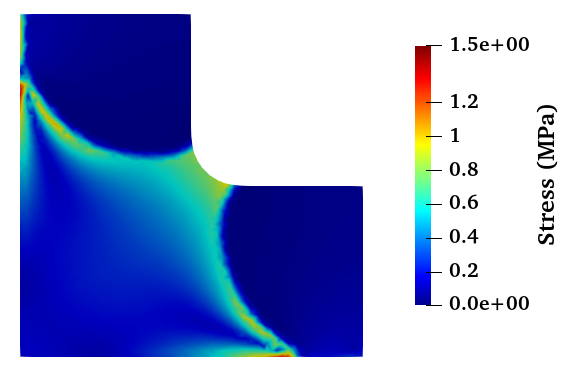
\includegraphics[width=0.44\linewidth]{Figures/Stress_VM_2.png}\vspace{0.2 in}\\
(a) \hspace{1.25 in} (b)
\caption{
Effect of the critical chance parameter $\alpha_c$ on the optimal design of the insulation component: (a) $\alpha_c=0.1$ and (b) $\alpha_c=0.4$. Each row displays the optimal design corresponding to different material porosity settings, along with the corresponding states (solid and fluid temperatures, solid displacement, and fluid pressure) and von Mises stress, all evaluated at the mean of the uncertain parameters $\overline{m}$.}
\label{fig:chance_result}
\end{figure}


\begin{figure}[h]
\centering
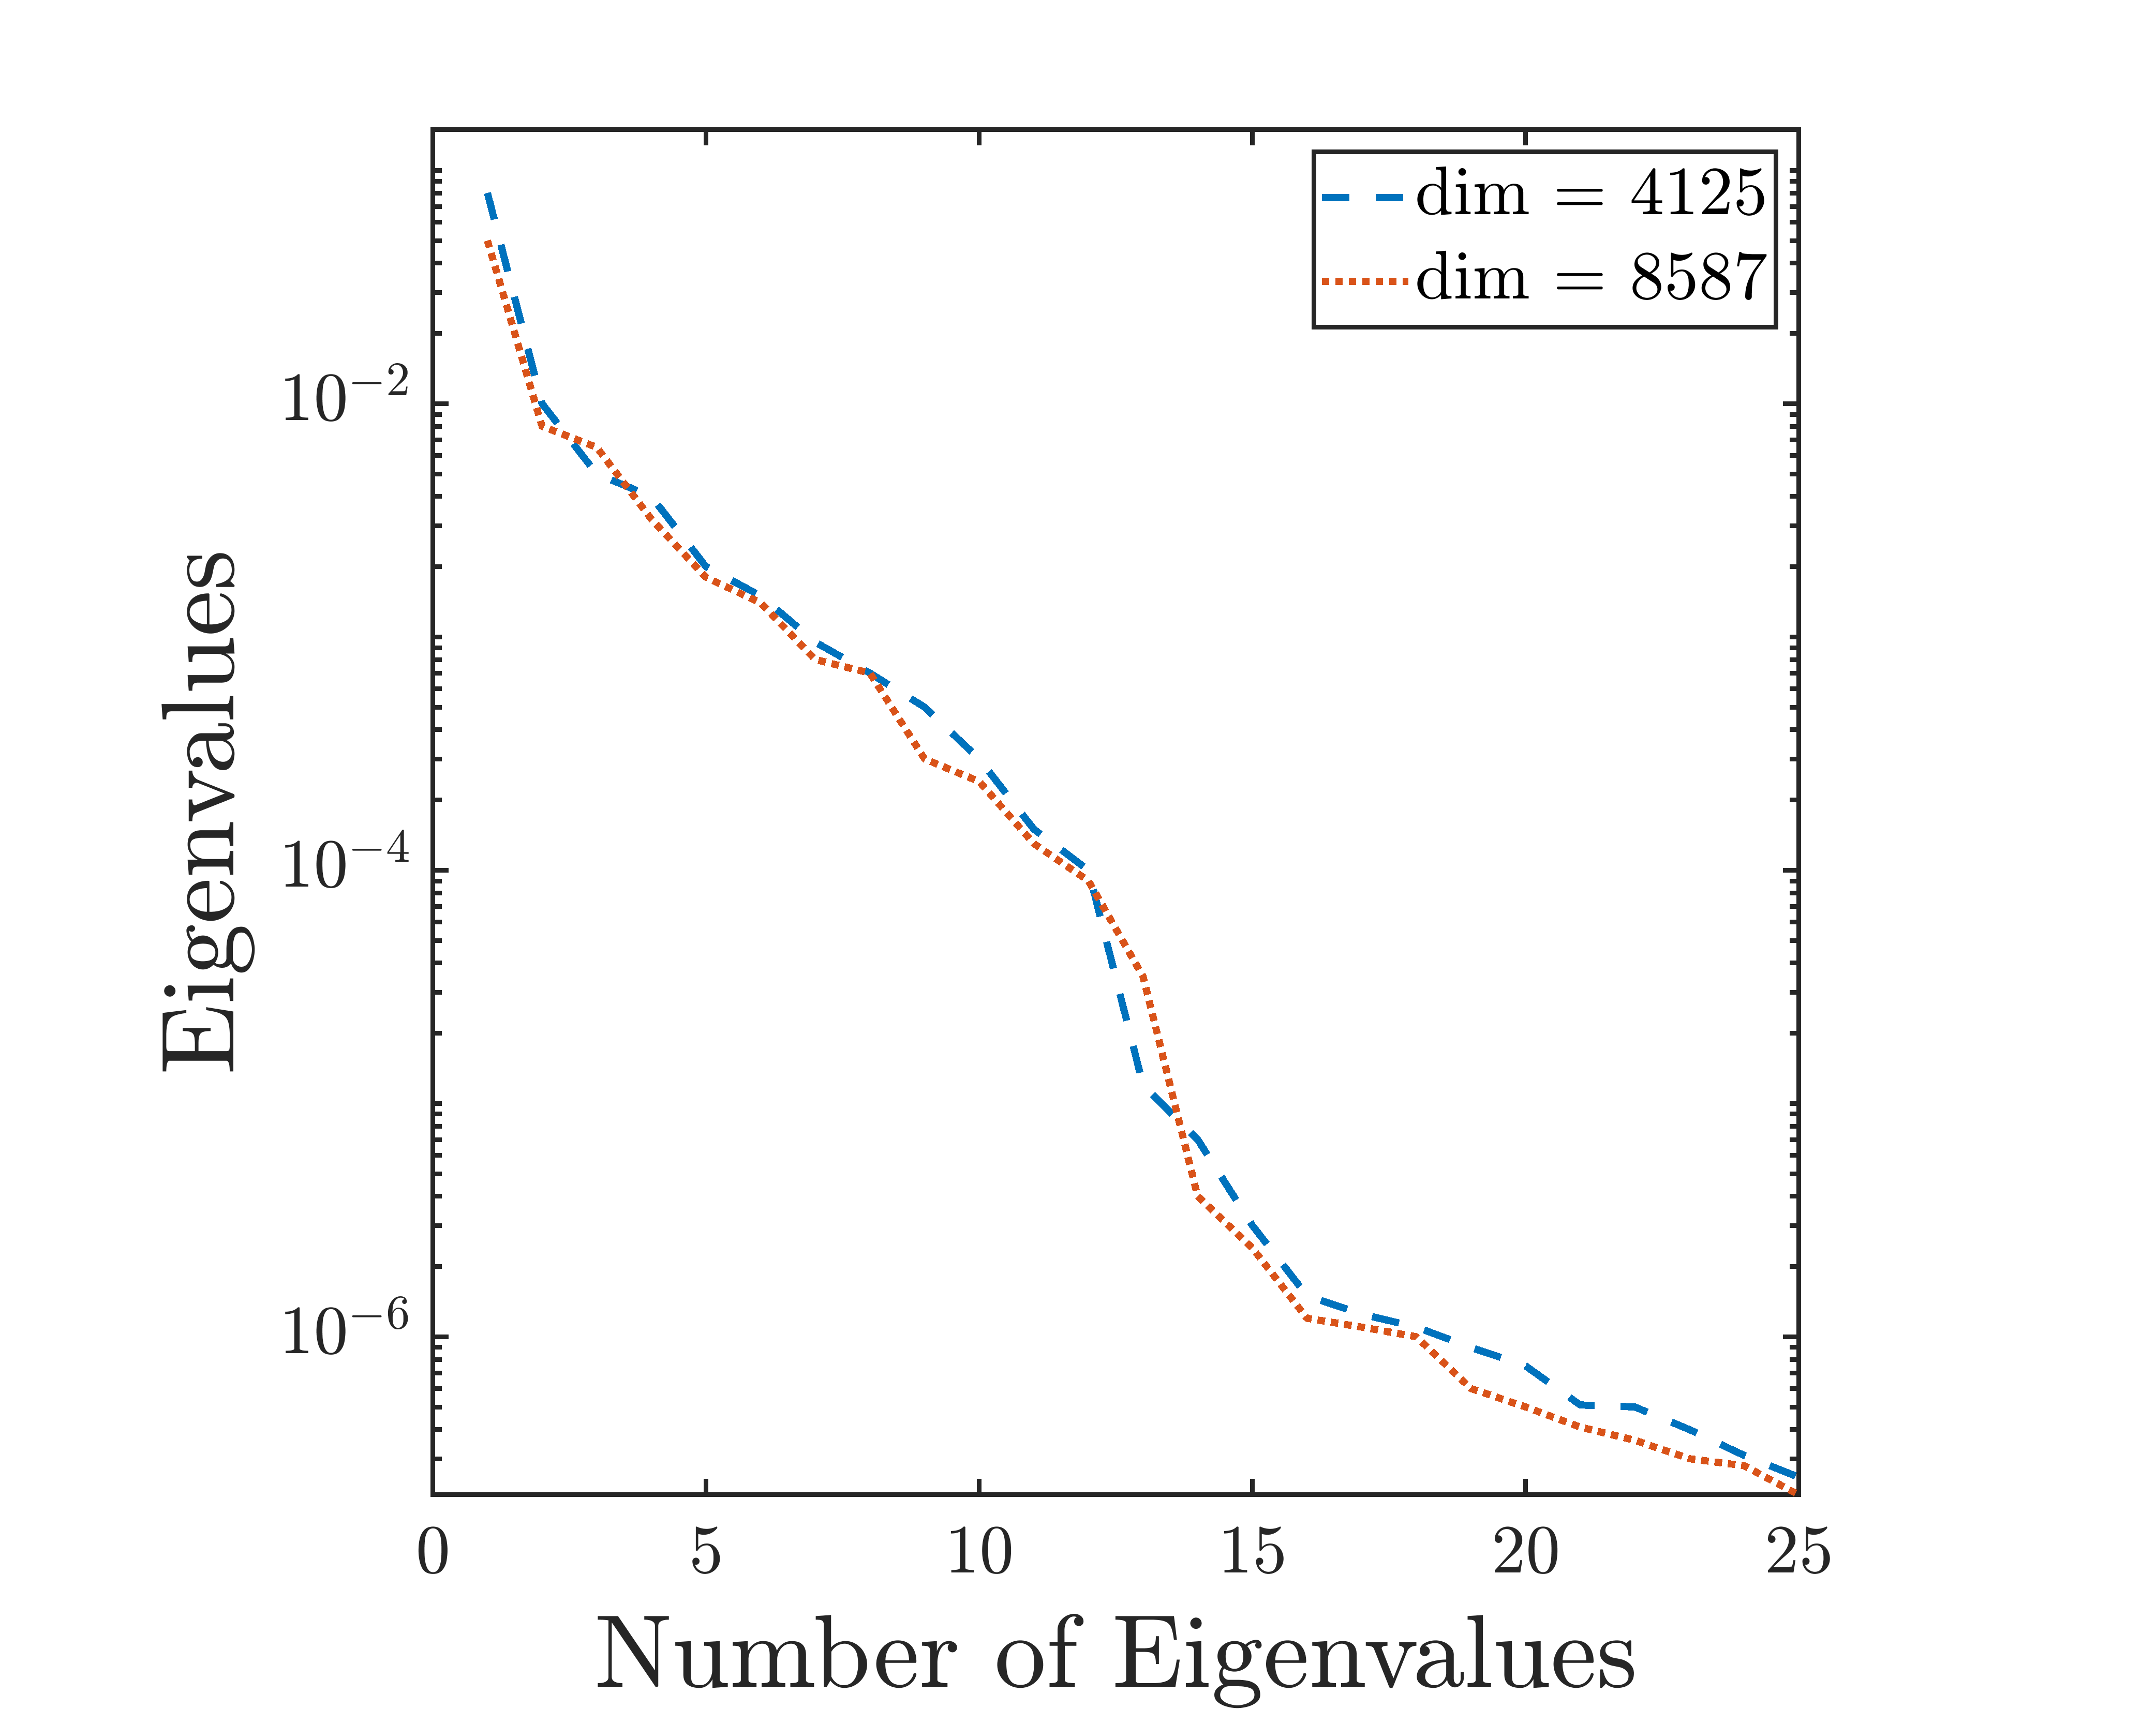
\includegraphics[width=0.8\linewidth]{Figures/Eigenvalue_1.png} 
\caption{Decay of the eigenvalues for the quadratic approximation with different uncertain parameter dimensions (mesh discretizations) indicating that the quadratic approximation results in a scalable design under uncertainty algorithm. \label{fig:eigenvalue}}
\end{figure}
In all numerical examples, a finite element mesh with 8587 nodes is utilized.
The proposed design under uncertainty framework is implemented leveraging a suite of open-source libraries, including FEniCS \cite{fenics} for finite element solution of the forward model, hIPPYLib \cite{VillaPetraGhattas16, VillaPetraGhattas18, VillaPetraGhattas21} for the trace estimator and Newton conjugate gradient algorithm, and SOUPy \cite{peng2022soupy} for quadratic approximation of the design objective.

\subsection{Scalability of the optimization algorithm}
\noindent Figure \ref{fig:eigenvalue} depicts the decay of eigenvalues in (\ref{eigen}) for various dimensions of design and uncertain parameters, denoting different finite element discretizations. The consistent nature of the eigenvalue decay across these dimensions underscores the scalability of the quadratic approximation with respect to the parameter dimension. In other words, the computational cost of the proposed design under an uncertainty framework is independent of the number of designs and uncertain parameters but rather depends on the low rank of the preconditioned Hessian.


\subsection{Effect of critical chance}
\noindent
The critical chance $\alpha_{c}$ represents the probability threshold beyond which the p-norm of von Mises stress may exceed the limiting critical stress. Therefore, $\alpha_{c}$ signifies the accepted degree of uncertainty in stress concentration to prevent mechanical failure of the insulation component.
Figure \ref{fig:chance_result} illustrates the optimal design results achieved by setting $\alpha_{c}$ to two distinct values. The limiting critical stress $T_{cr}$ for both cases is 1.6 MPa. Additionally, this figure presents the corresponding states, and von Mises stress assessed at the mean of the uncertain parameters. The findings suggest that considering a higher critical chance entails the placement of mechanically stronger material (shown in red) over a broader region of the domain, resulting in diminished local stress values across the component. However, enhancing stability with higher $\alpha_{c}$ values will come at the expense of the insulation performance of the component, as evidenced by the probability distribution of thermal compliance depicted in Figure \ref{fig:chance_thermal}.



\subsection{Effect of Tikhonov weight}
\noindent
Next, we explore the impact of Tikhonov regularization by considering two different weights: $\beta_{tik} = 1 \times 10^{-4}$ and  $\beta_{tik} = 2 \times 10^{-4}$, depicted in Figure \ref{fig:Tikhonov}. 
As illustrated in this figure, stronger regularization yields smoother optimal design solutions within the domain, resulting in increased interface thickness between the two materials. For more intricate problems, it may be necessary to enhance regularization to achieve a nearly sharp interface \cite{tan2024scalable}.

\begin{figure}[h]
\centering
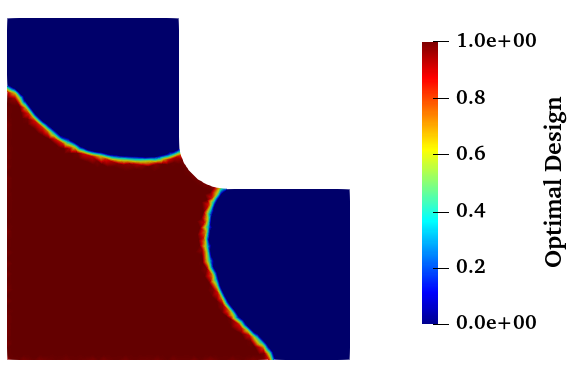
\includegraphics[width=0.44\linewidth]{Figures/Tikhonov_1.png} ~  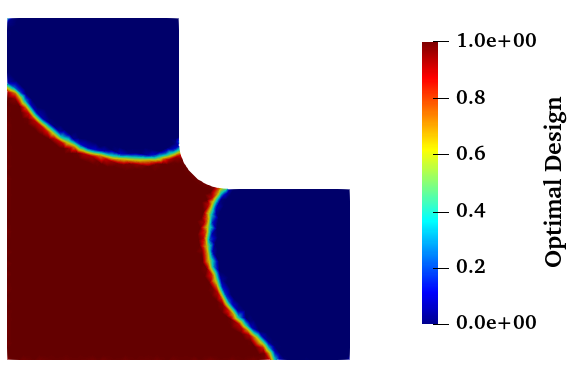
\includegraphics[width=0.44\linewidth]{Figures/Tikhonov_2.png}\\
(a) \hspace{1.3 in} (b)\\
\caption{Effect of Tikhonov weight on the optimal design solutions: (a) $\beta_{\text{tik}} = 1 \times 10^{-4}$ and (b) $\beta_{\text{tik}} = 2 \times 10^{-4}$}\label{fig:Tikhonov}
\end{figure}

\subsection{Effect of smoothing  and penalty parameter}
We demonstrate the effect of the scaling parameters $\sigma_{\beta}$ and $\sigma_{\gamma}$. The effect of scaling parameter $\sigma_{\beta}$ is demonstrated in two cases. As the smoothing parameter $\beta$ increases, the approximation to the indicator function becomes more accurate, and hence the solution starts to improve. Figure \ref{fig:beta} shows the convergence of the value of chance $l_{\beta} f$ for two different values of scaling parameter $\sigma_{\beta}$ while keeping the other parameters constant. The convergence of $l_{\beta} f$ is observed with an increasing number of iterations $k$ in Algorithm 1. When the value of $\sigma_{\beta}$ is higher, the value of computed chance $l_{\beta}$ is much closer to the value of critical chance $\alpha_{c} = 0.1$. 
As the scaling factor for penalty parameter $\sigma_{\gamma}$ increases, the violation of critical chance $\alpha_{c}$ is strongly penalized, and it leads to a reduction in the number of function calls required to attain convergence. Here, the number of functional calls refers to the number of times the function inside the Newton CG algorithm is evaluated for computing the gradient and the hessian. The number of function calls is related to the computational cost. If the number of function calls is high, then the computational cost is also high, and vice-versa. We analyze the effect of scaling parameter $\sigma_{\gamma}$ on the number of function calls for the optimization problem (\ref{eq: optimization_penalty}). Figure \ref{fig:gamma} shows the reduction in the number of functional calls with an increasing number of iteration $k$ as we closely move towards the optimal solution $d_{\text{opt}}$, as explained for Algorithm 1. As illustrated in Figure \ref{fig:gamma}, the number of function calls required for $\sigma_{\gamma}=1000$ is less as compared to $\sigma_{\gamma}=100$. This shows that stronger penalization leads to faster convergence for obtaining the optimal solution $d_{\text{opt}}$, with less number of function calls.


\begin{figure}[h]
\centering
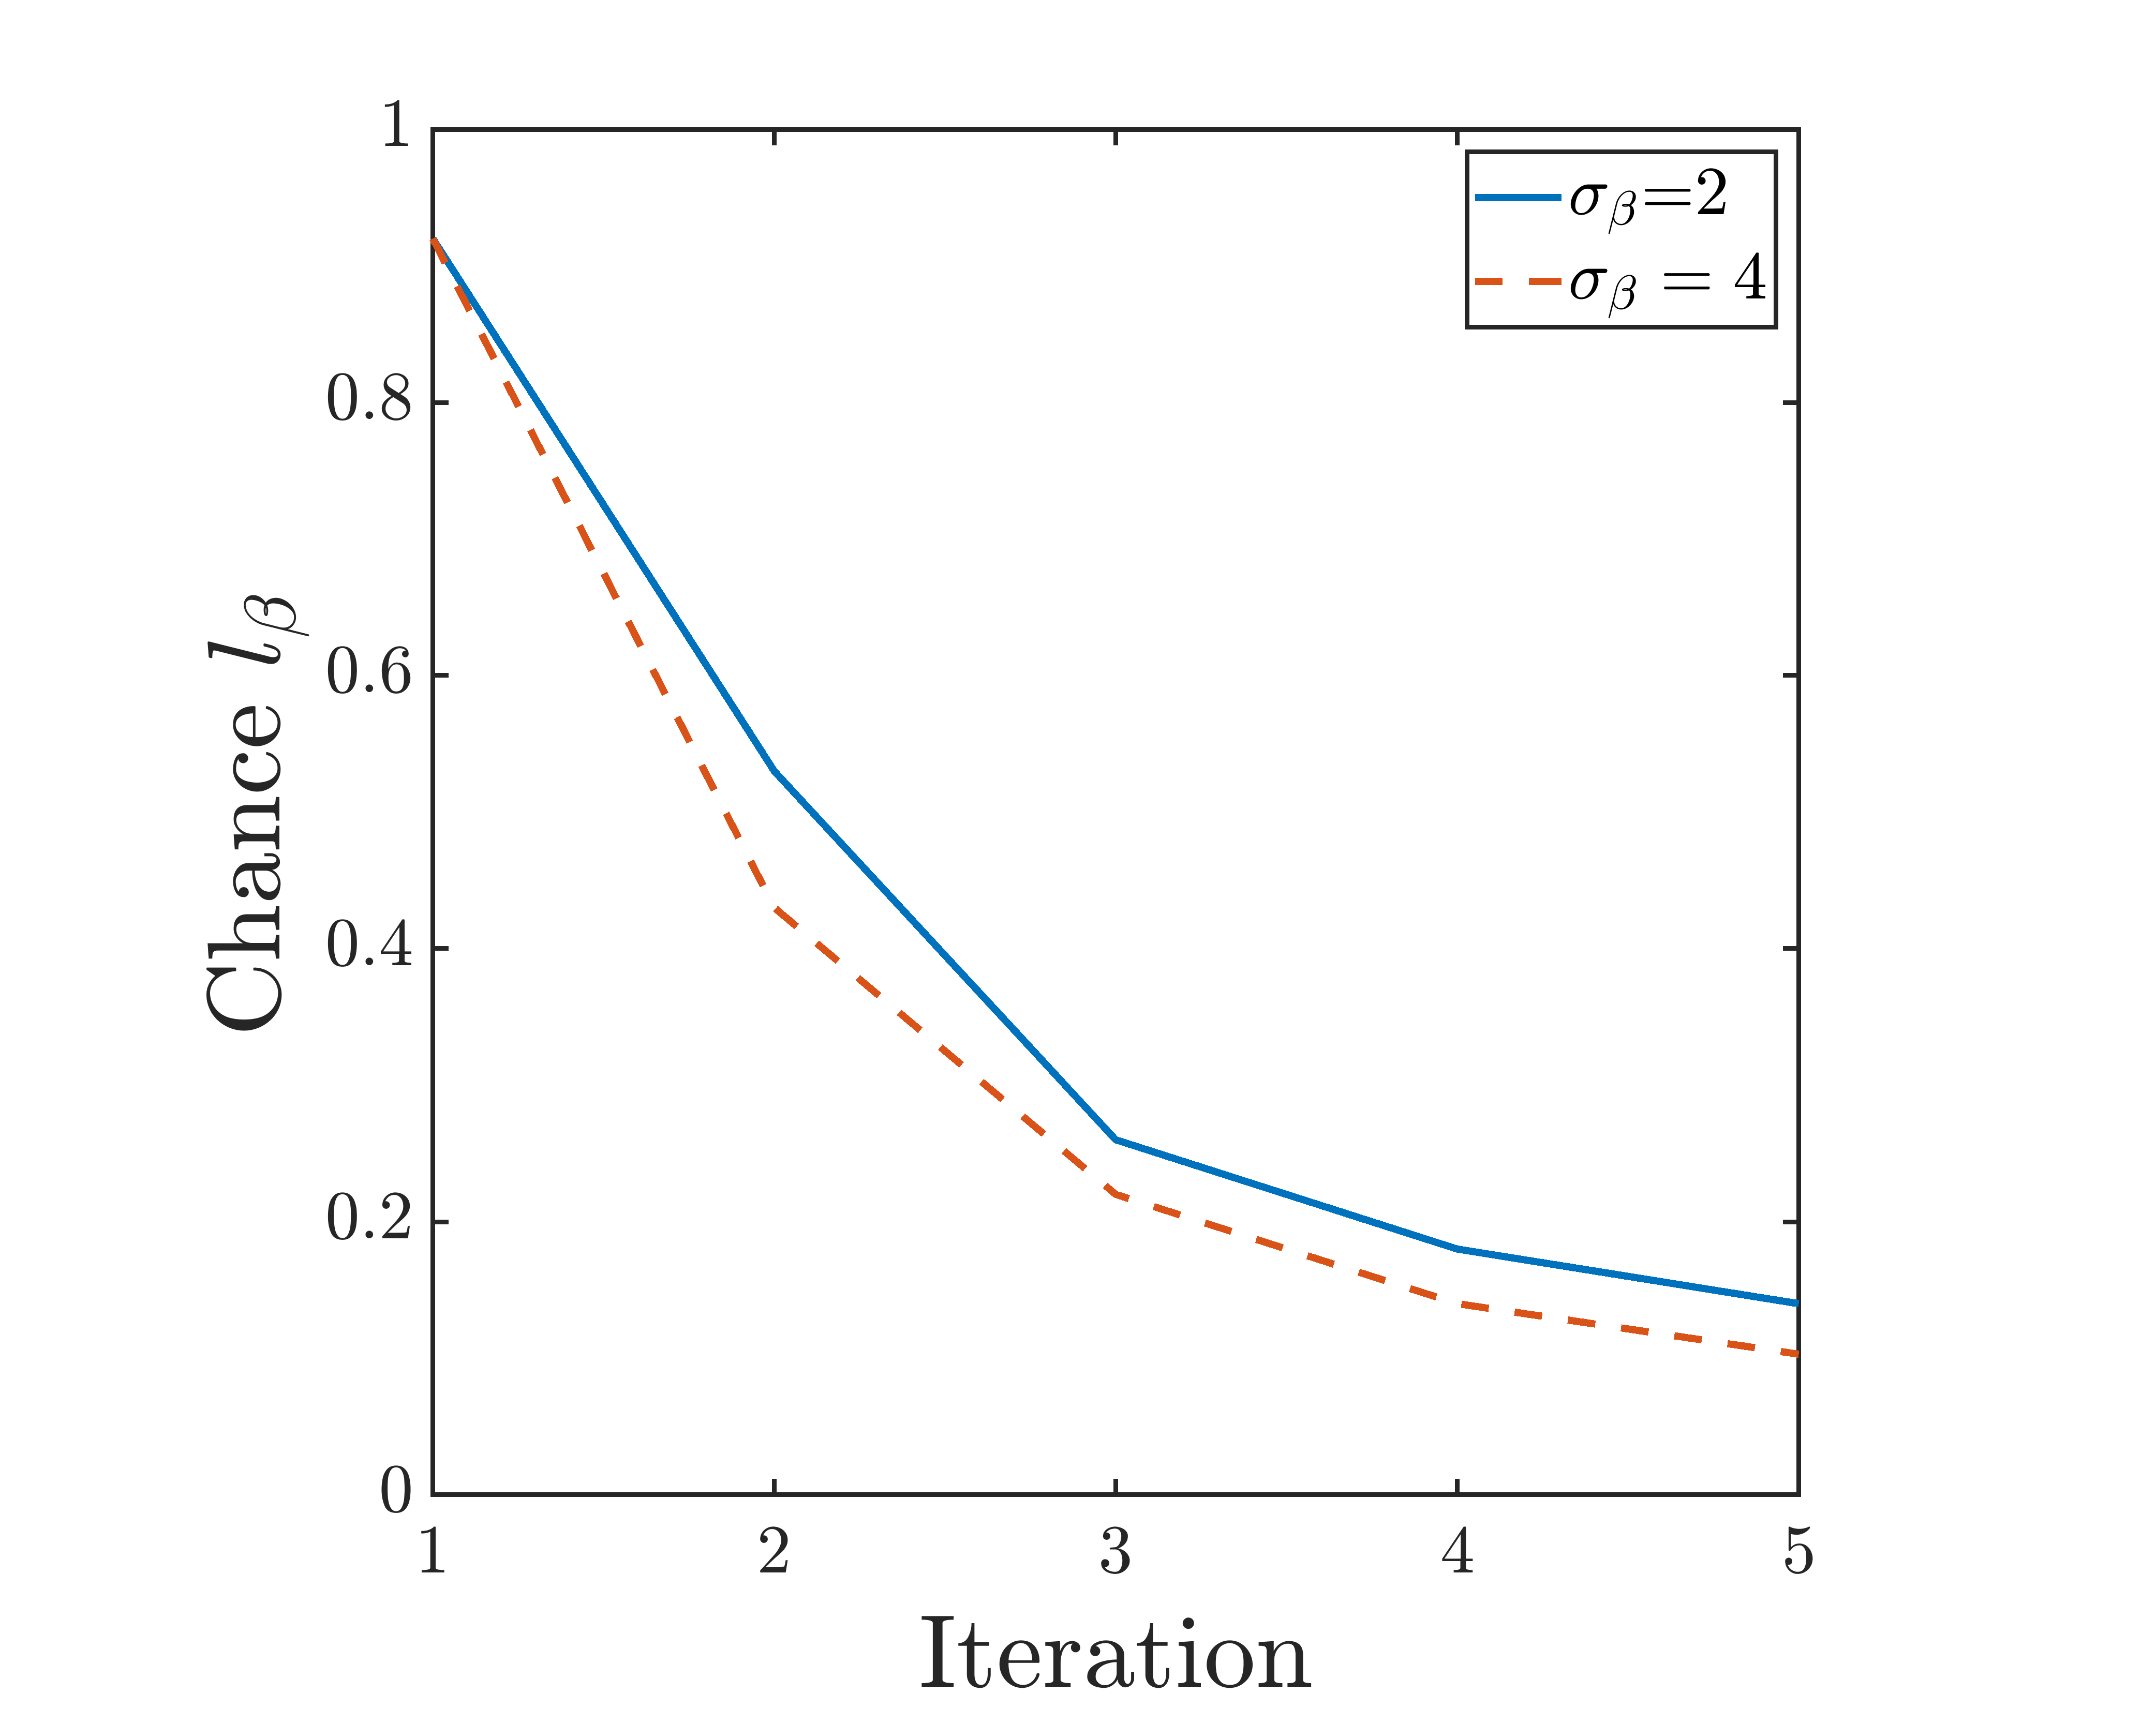
\includegraphics[width=0.8\linewidth]{Figures/Beta_1.png}
\caption{Effect of parameter $\sigma_{\beta}$ on the convergence of the value of chance.}\label{fig:beta}
\end{figure}
\begin{figure}[h]
\centering
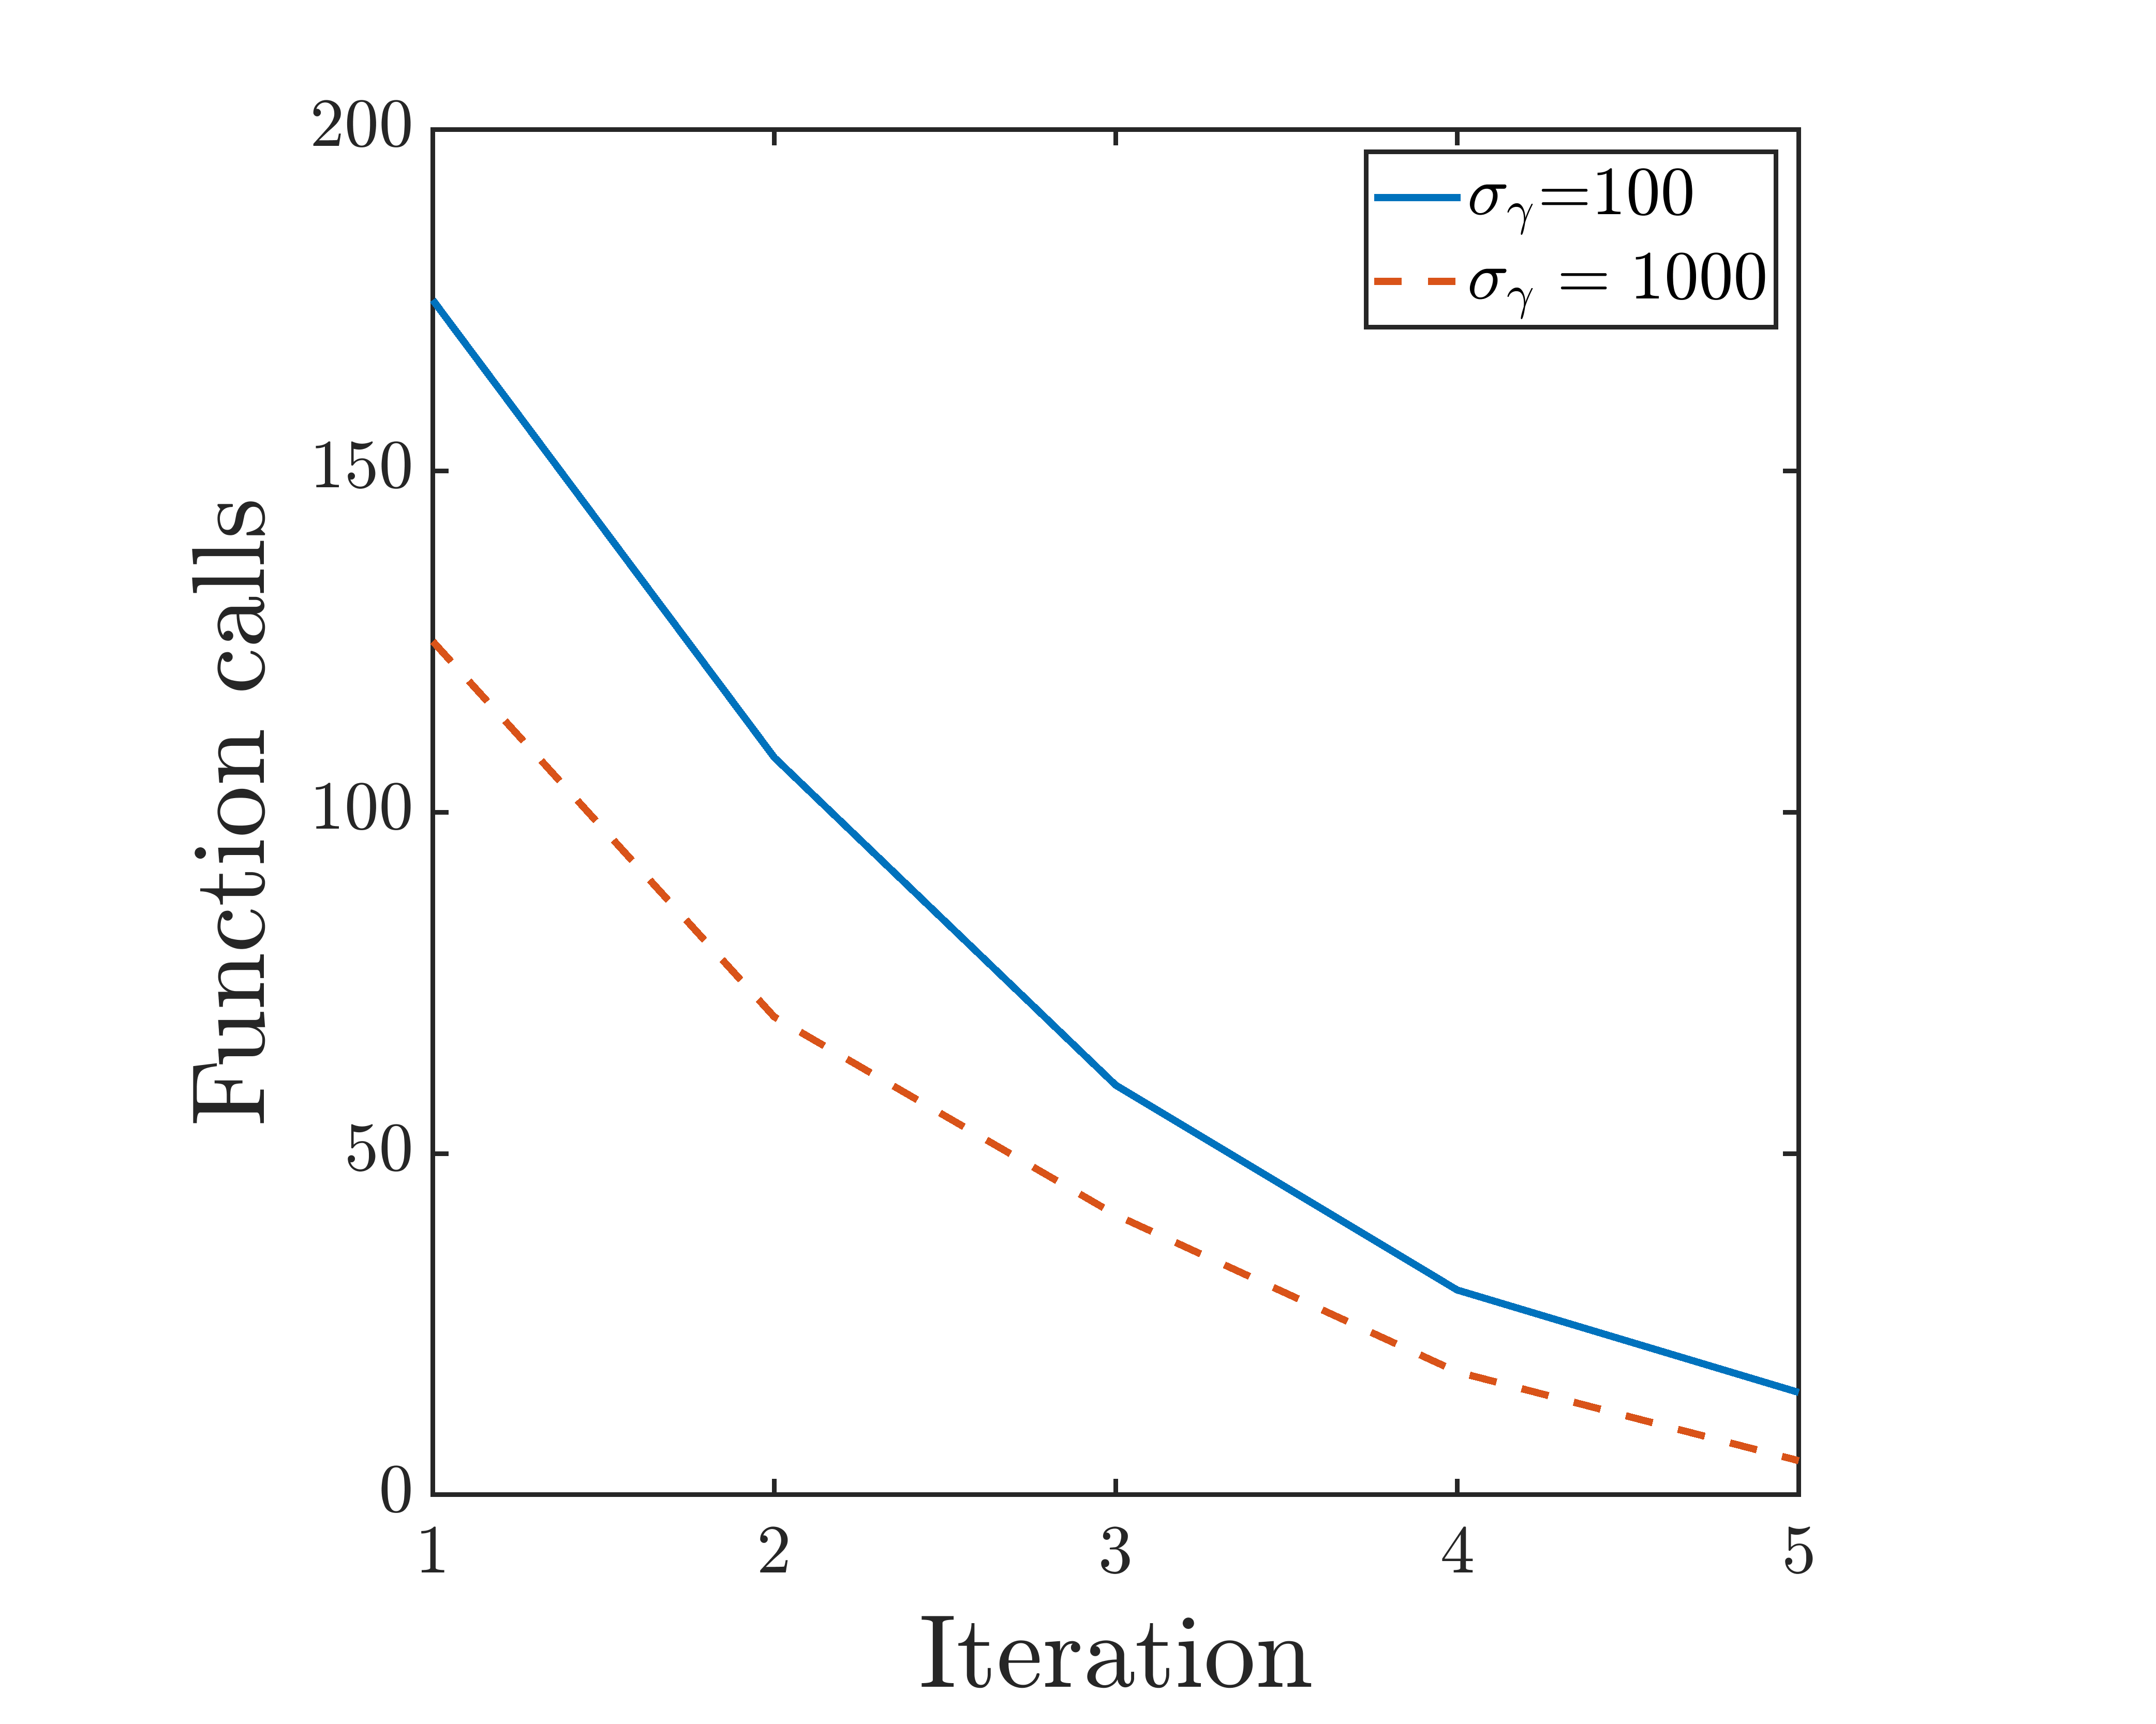
\includegraphics[width=0.8\linewidth]{Figures/Gam_1.png}
\caption{Effect of parameter $\sigma_{\gamma}$ on the reduction
in the number of functional calls with an increasing number of
iteration.}\label{fig:gamma}
\end{figure}

\section{Conclusions}
\noindent
This paper presents an efficient and scalable computational framework for chance-constrained optimal design under high-dimensional uncertainty for systems governed by PDEs. To capture spatially correlated uncertainty, a Gaussian random field with a Matern covariance kernel is utilized, requiring the solution of a stochastic PDE.
To address challenges posed by high-dimensional parameter spaces, an approximation method is proposed to solve the resultant optimization problem, ensuring computational cost remains invariant to the number of design parameters. To handle discontinuous indicator functions and inequality constraints, a smooth approximation and a penalty method within a continuation Newton conjugate gradient algorithm are taken into account.

%

The framework is applied to the design of thermal insulation components in building envelopes utilizing silica aerogel porous materials. The material behavior is governed by a thermo-mechanical model of aerogel based on the continuum theory of mixtures. The design parameter of interest is the spatial distribution of porosity across the domain, inherently exhibiting uncertainty due to material variations and fabrication errors.
The cost functional comprises the mean of thermal insulation properties, with chance constraints imposed on the optimization problem to limit the maximum von Mises stress in the domain below a specified threshold, to prevent mechanical failure due to excessive stress. Application of the proposed framework to the design of building insulation components aims to achieve both thermal insulation and mechanical stability. The impact of critical chance, limiting critical stress value, Tikhonov regularization weight, smoothing, and penalty parameters on the designed spatial distribution of material porosity and corresponding thermal and mechanical performances is investigated. The results highlight the efficacy of the proposed design under uncertainty framework, offering orders of magnitude reduction in computational cost compared to sampling-based methods for handling the design objective moments and constraints.
In future work, the proposed method will be expanded to account for uncertainty in material model parameters, characterized via Bayesian model calibration, e.g., \cite{tan2022predictive, liang2023bayesian, tan2022toward, lima2021bayesian, tan2021predictive} using experimental measurements of thermal and mechanical properties of silica aerogel, e.g., \cite{an2021wearable}.



\bibliographystyle{asmeconf}  %% .bst file following ASME conference format. Do not change.
\bibliography{references}
\end{document}

